\section{Browser Warnings and HTTPS Errors}
%����Ҫ��дһ���ܽ���ܵĻ�
\subsection{Browser Security Warnings}
Browser security warnings protect users against various network attacks,
    and we only consider the MitM or impersonation attacks in HTTPS.
The  attacks may be launched
     by using a forged or revoked certificate,
    or deceiving users to visit the website through plain HTTP.
When such errors happen,
    a browser shows the warnings in different ways to ensure security while minimize the side effects of user experience,
    because an HTTPS error is not definitely caused by the attacks.

% We describe security warnings of major browsers.


\subsubsection{Low-risk warning}
For low-risk errors, it shows a security indicator \emph{not interrupting the user's browsing}.
For example, as shown in Figure \ref{fig-a},
    the browser changes the HTTPS lock icon into a warning indicator in the address bar,
     and shows a hint when the user clicks the icon.
%In this scenario, a passive security indicator indicates minor HTTPS errors by removing lock icon, changing lock icon��s color, providing textual information, or by other means without interrupting the user��s browsing.
%This is probably because webmaster has configured his website correctly, including purchasing a valid certificate, but the website still contains images or scripts over plain HTTP.
%Although the browser was able to establish a valid HTTPS connection, there are still minor problems.
On low-risk errors, the browser still establishes HTTPS connections with the website. %Fig. 1 shows the Low-risk warning in Chrome.  connections with the visited website. Fig. 1 shows the Low-risk warning

%\textcolor[rgb]{1.00,0.00,0.00}{
%    Chrome displays the visited website with a passive indicator .
%    The passive indicator is a popupdialog box which explains the cause of the warning.
%    However, it does not give the user any choice, nor gives the user any recommendation, nor does it affect the user's access to the website.}

\begin{figure}[htb]
%\setlength{\belowcaptionskip}{-2cm}
%\centerline{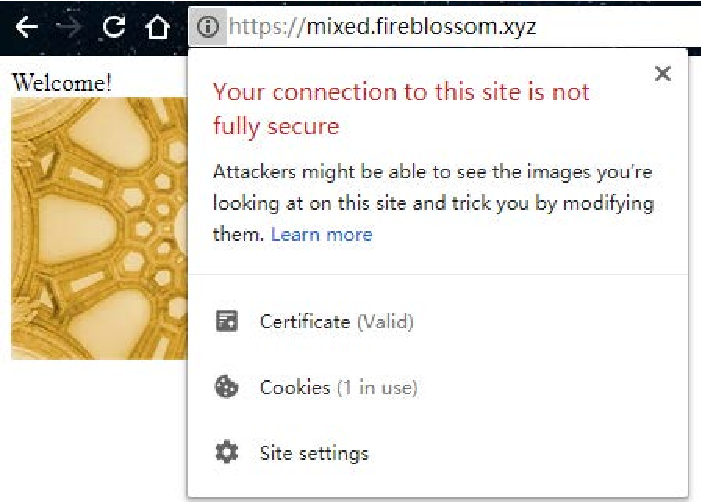
\includegraphics[height=2.4cm,width=7cm]{Figure/fig1.pdf}}% �ǵû���chrome�Ľ�ͼ
\centerline{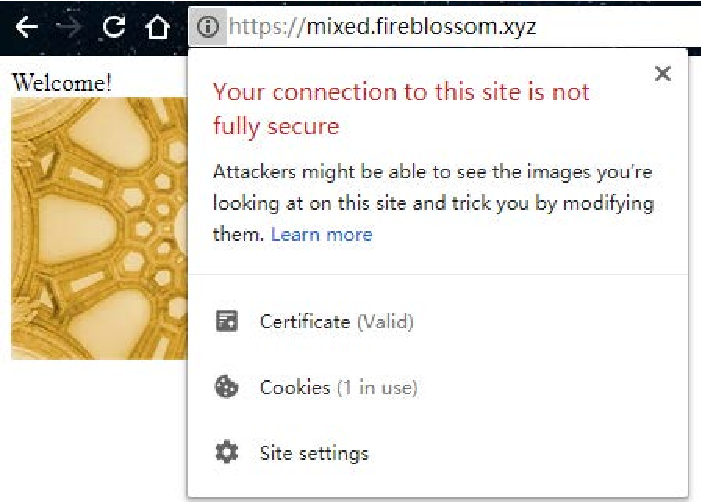
\includegraphics[scale=0.49]{Figure/fig1.pdf}}
%\centerline{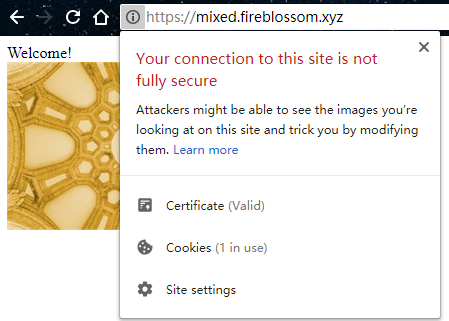
\includegraphics{Figure/fig1.eps}}
\centering
\caption{Low-risk (Level-A) warning in Chrome.}
\label{fig-a}
\end{figure}


\subsubsection{Medium-risk warning}
For medium-risk errors, it shows a \emph{bypassable warning} that discourages users from continuing.
For example, as shown in Figure \ref{fig-b},
    the browser stops the webpage load and displays a full-screen warning with options: ``Back to safety'' and ``Proceed to this website (unsafe)''.
The security errors are explained in this page.
If the user bypasses (or clicks through)
     the warning by clicking ``Proceed to this website (unsafe)'',
     HTTPS connections are established.
%For medium-risk errors, it will show a bypassable warning that discourages the user from continuing.
%Bypassable HTTPS security warnings are the most common type of browser warning. Browsers use bypassable HTTPS security warning to treat the vast majority of HTTPS errors.


%\textcolor[rgb]{1.00,0.00,0.00}{
%Chrome presents the user with the title "Your connection is not private",
%    Primary text "Attackers might be trying to steal your information from example.com (for example, passwords, messages, or credit cards)",
%    button "Advanced",
%    and button "Bsck to safety".
%A more technical explanation about the cause of the error
%    are hidden in "Advance" section.
%That is,
%    users can click on "Advanced"to seek more information about the specific error
%    and reveal the link to proceed.}

\begin{figure}[!h]
%\setlength{\belowcaptionskip}{-2cm}
%\centerline{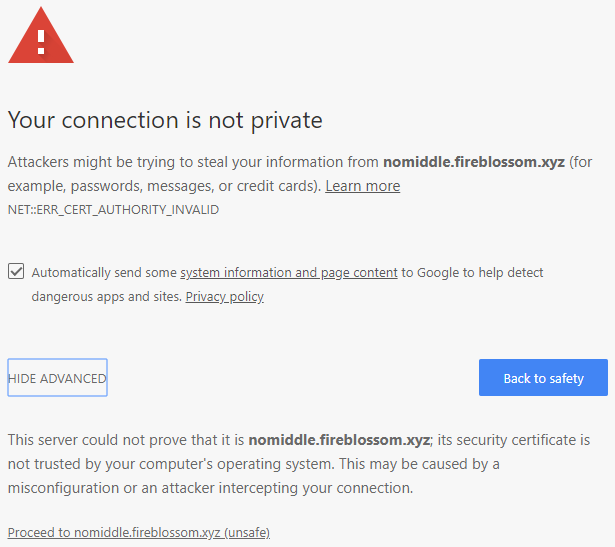
\includegraphics[scale=0.4]{Figure/fig2.png}}
\centerline{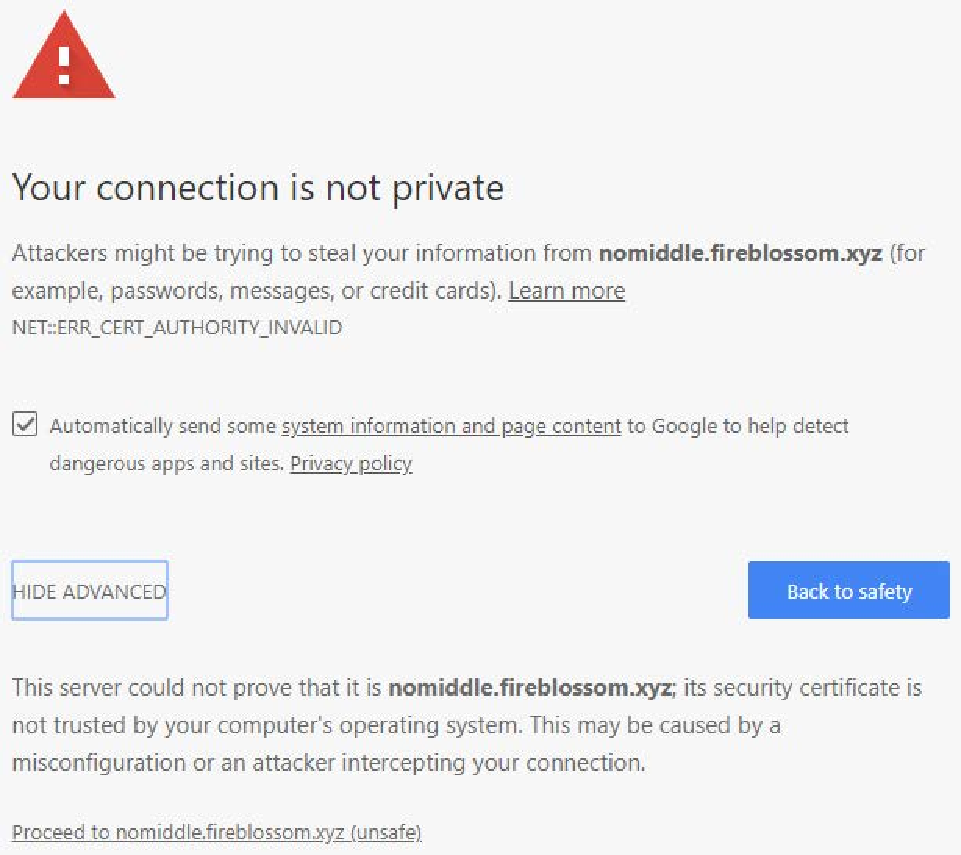
\includegraphics[scale=0.36]{Figure/fig2.pdf}}
\caption{Medium-risk (Level-B) warning in Chrome.}
\label{fig-b}
\end{figure}
%In this scenario, if there is an HTTPS error, the browser will stop the page load and display an HTTPS security warning explaining the cause of the error. Typically, users are able to click through the warning by clicking on a button, but this may be disabled if the website servers the HTTP Strict Transport Security (HSTS) or HTTP Public Key Pinning (HPKP) header. Although the HTTP(s) traffic we captured through Fiddler[ https://www.telerik.com/fiddler] shows the web page is not transmitted in plain text, clicking through the warning may allow an actual man-in-the-middle attack to proceed.


\subsubsection{High-risk warning}
For high-risk errors, it shows a \emph{non-bypassable warning to stop the browsing}.
For example,
    the browser displays a full-screen webpage explaining the error,
     with a button to \emph{retry}.
As shown in Figure \ref{fig-c},
    different from the medium-risk one,
    a high-risk warning does not provide the option ``Proceed to this website (unsafe)''.
On high-risk errors,
    the browser closes HTTPS connections to the visited server.

%For high-risk errors, it will show a security warning that the user cannot bypass.
%As a worst case scenario, the browser will prevent uses from continuing to browse the website by showing a security warning that the users cannot bypass.

%\textcolor[rgb]{1.00,0.00,0.00}{Similar to the medium-risk warning in the post,
%    The high-risk warning in Chrome shows a title, a primary body text, a hidden detailed explanation in "Advanced".
%    However, users can only reload, and cannot bypass the warning.}

\begin{figure}[htbp]
%\setlength{\belowcaptionskip}{-2cm}
%\centerline{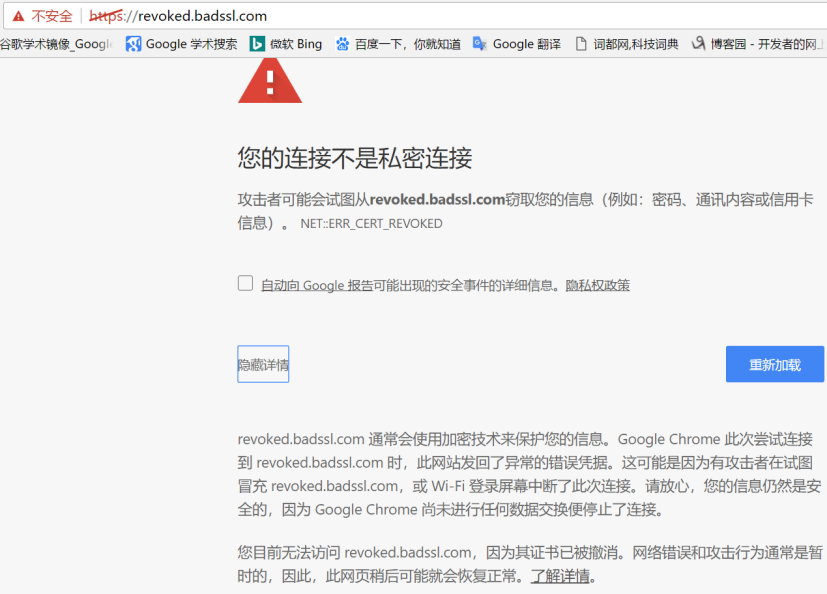
\includegraphics[scale=0.4]{Figure/fig3.png}}% �ǵû����Լ�fireblossom.xyz��ַ�Ľ�ͼ
%\centerline{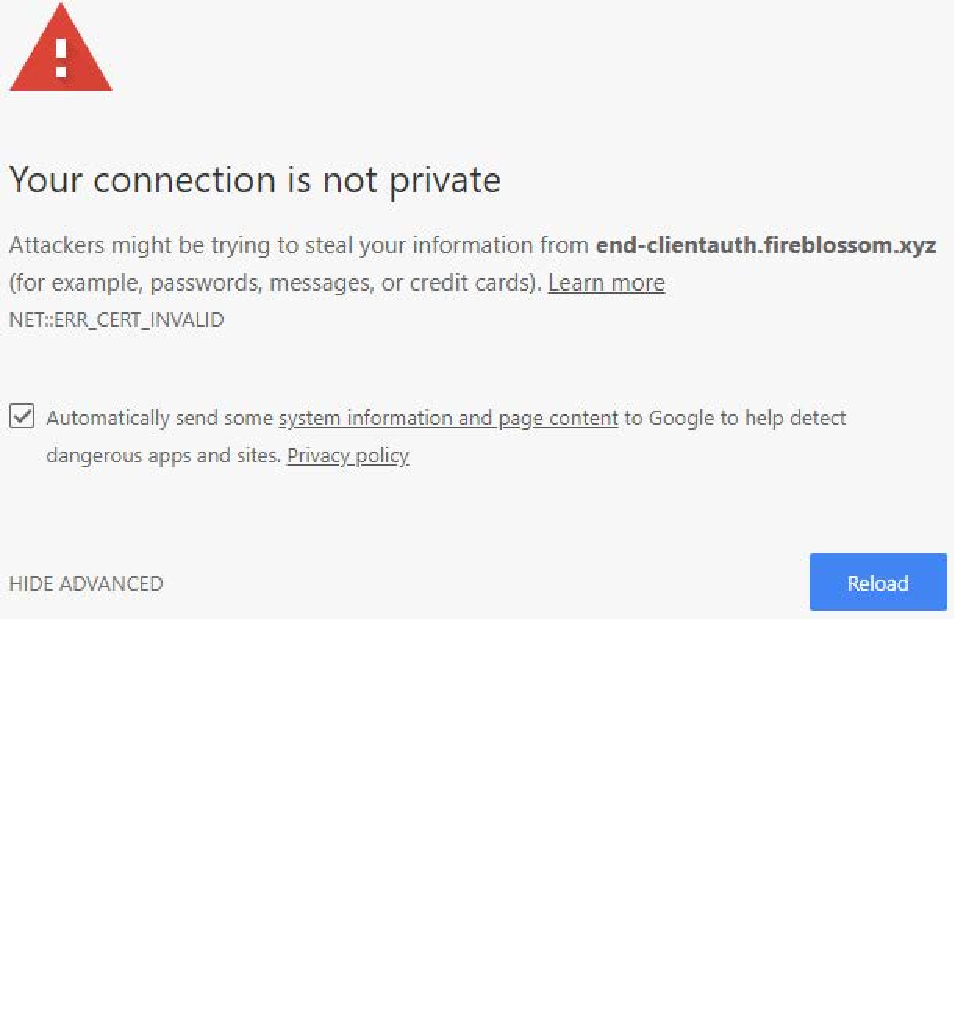
\includegraphics[height=6.58cm,width=6.11cm]{Figure/fig3.pdf}}
\centerline{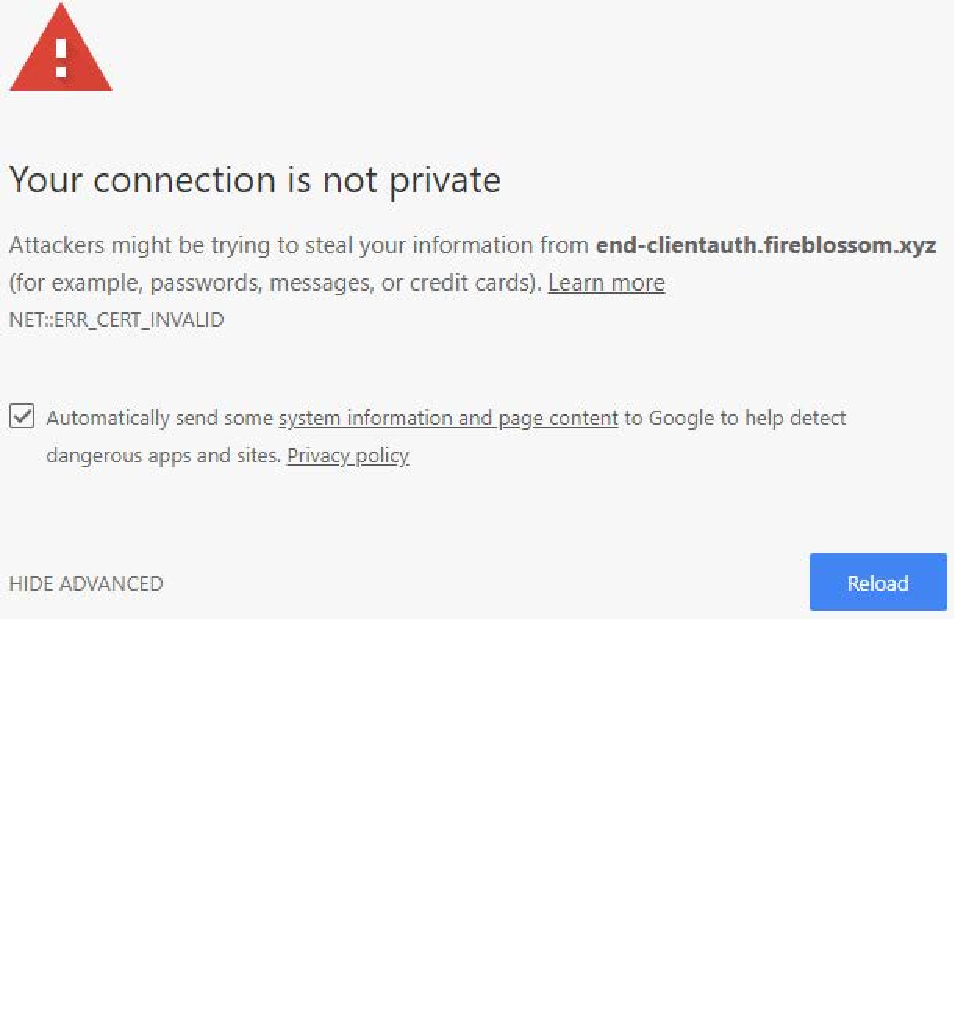
\includegraphics[scale=0.37]{Figure/fig3.pdf}}
%\centerline{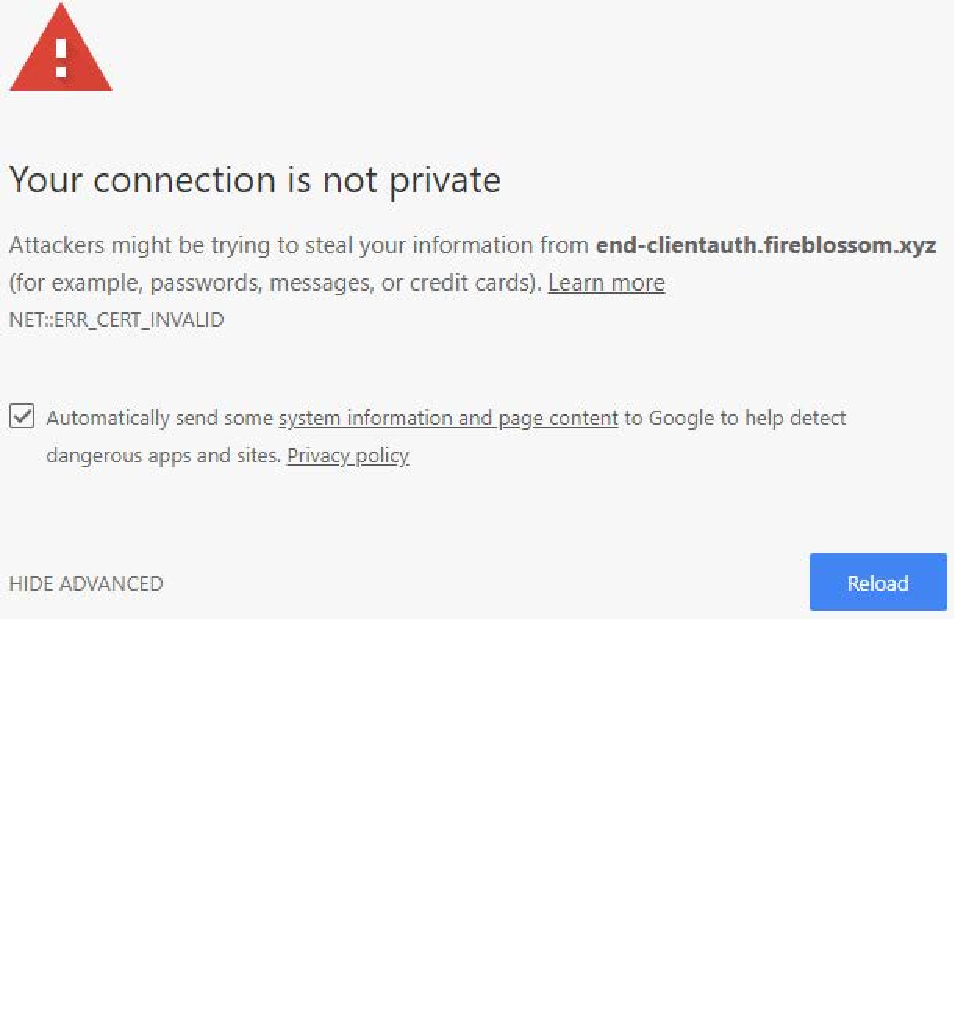
\includegraphics[height=4.656cm,width=7.188cm]{Figure/fig3.pdf}}
\caption{High-risk (Level-C) warning in Chrome.}
\label{fig-c}
\end{figure}
%this is probably because the website is supposed to establish a valid HTTPS connection, but the certificate chain fails to validate (e.g., a HTTPS certificate error occurs in a website that has deployed HSTS policy).




\subsubsection{Fatal warning}
On fatal errors, it \emph{immediately closes the connections} and stops the browsing.
%For example,
 %   the browser displays a full-screen fatal warning,
  %   discouraging any retrying.
%On fatal errors,
%    the browser immediately closes HTTPS connections to the server.
Such warnings are shown when it is impossible to establish HTTPS connections,
    for example, due to unsupported protocol versions or algorithms.


%For fatal errors, it shows a warning stop uses' browsing.
%The browser may fail to establish a HTTPS connection to the server for unsupported TLS version, cipher mismatch, or other reasons.
%In this scenario, the browser cannot obtain certificates from the web server, let alone certificate validation, so the TLS handshake error is not discussed in this paper.
%\begin{figure}[htbp]
%\centerline{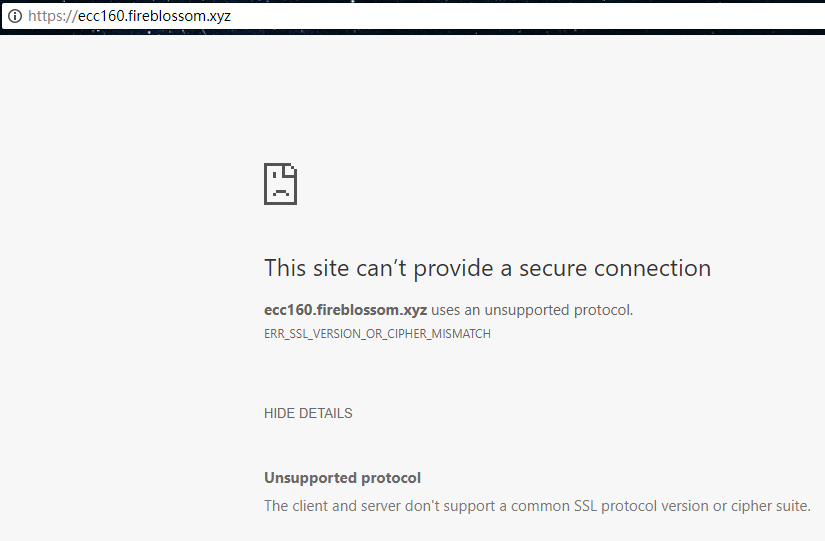
\includegraphics[height=3cm,width=7cm]{Figure/fig4.png}}% ��ͼ��Ҫ�ٵ�����������
%\caption{Fatal warning in Chrome.}
%\label{fig-d}
%\end{figure}
%Warning Images
